%!TEX root = ../../thesis.tex

\section{Reading Comprehension vs. Question Answering}
\label{sec:rc-qa-diff}

There is a close relationship between reading comprehension and question answering.  We can view reading comprehension as an instance of question answering because it is essentially a question answering problem over a short passage of text. Nevertheless, although reading comprehension and general question answering share many common characteristics in problem formulation, approaches and evaluation, we think they emphasize different thing as their final goals:

\begin{itemize}
    \item
        The ultimate goal of question answering is to build computer systems which are able to automatically \ti{answer questions} posed by humans, no matter what sort of resources they depend on. These resources can be structured knowledge bases, unstructured text collections (encyclopedias, dictionaries, newswire articles and general Web documents), semi-structured tables or even other modalities. Towards the better performance of QA systems, a lot of efforts have been put into (1) how to search and identify relevant resources, (2) how to integrate answers from different pieces of information, or even (3) to study what types of questions humans usually ask in the real world.
    \item
        However, reading comprehension puts more emphasis on \ti{text understanding} with answering questions regarded as a way to measure language understanding. Therefore it requires a deep understanding of the given passage in order to answer the question. Due to this key difference, early works in this field mostly focused on fictional stories ~\cite{lehnert1977process} (later extended to Wikipedia or Web documents), so all the information to answer comprehension questions comes from the passage itself instead of any world knowledge. The questions are also specifically devised to test different aspects of text comprehension. This distinction is akin to what questions people usually ask on search engines versus what sorts of questions are usually posed in human reading comprehension tests.
\end{itemize}

Similarly, early work \cite{mitchell2009populating} used the terms \tf{micro-reading} and \tf{macro-reading} to differentiate these two scenarios. Micro-reading focuses on reading a single text document and aims to extract the full information content of that document (similar to our reading comprehension setting), while macro-reading takes a large text collection (e.g., the Web) as input and extracts a large collection of facts expressed in the text, without requiring that every single fact is extracted. Macro-reading can effectively leverage the \ti{redundancy} of information across documents by focusing on analyzing simple wordings of the fact in the text, while macro-reading has to investigate deeper level of language understanding.

This thesis mostly focuses on reading comprehension. In Chapter~\ref{chapter:openqa}, we will come back to more general question answering problems, discuss its related work and also demonstrate that reading comprehension can be also helpful in building question answering systems.

\section{Datasets and Models}
\label{sec:rc-drive}


As seen in Section~\ref{sec:deep-learning-era}, the recent success of reading comprehension has been mainly driven by two key components: \ti{large-scale reading comprehension datasets} and \ti{end-to-end neural reading comprehension models}. They work together to advance the field and push the boundaries of building better reading comprehension systems:

\begin{description}
\item
On the one hand, the creation of large-scale reading comprehension datasets has made it possible to train neural models, while demonstrating their competitiveness over symbolic NLP systems. The availability of these datasets further attracted a lot of attention in our research community and inspired a series of modeling innovations. Tremendous progress has been made thanks to all these efforts.
\item
On the other hand, understanding the performance of existing models further helps identity the limitations of existing datasets. This motivates us to seek better ways to construct more challenging datasets, towards the ultimate goal of machine comprehension of text.
\end{description}


\begin{figure}[!t]
    \center
    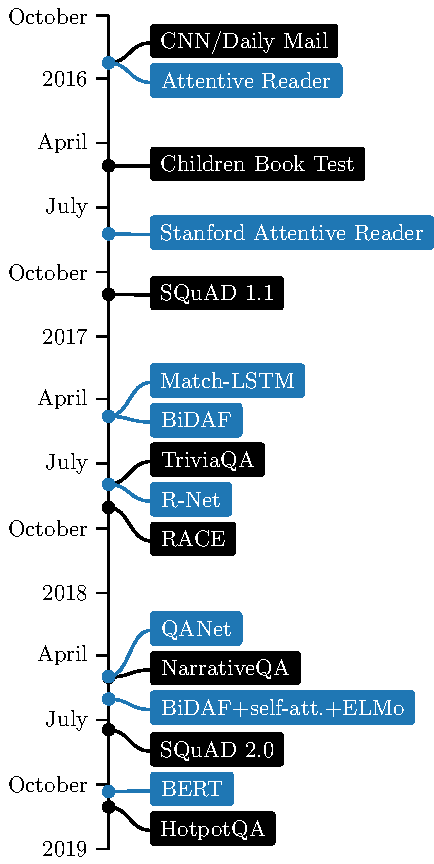
\includegraphics[scale=1.0]{img/timeline.pdf}
    \longcaption{The recent development of datasets and models in neural reading comprehension}{\label{fig:timeline}The recent development of datasets (black) and models (blue) in neural reading comprehension. For the timeline, we use the date that the corresponding papers were published, except \sys{BERT}~\cite{devlin2018bert}.}
\end{figure}

Figure~\ref{fig:timeline} shows a timeline of the recent development of key datasets and models since 2016. As is seen, although it has been only 3 years, the field has been moving strikingly fast. The innovations in building better datasets and more effective models have occurred alternately and both contributed to the development of the field. In the future, we believe it will be equally important to continue to develop both components.

In the next chapter, we will mainly focus on the modeling aspect, using the two representative datasets that we described earlier: \sys{CNN/Daily Mail} and \sys{SQuAD}. In Chapter~\ref{chapter:rc-future}, we will discuss more about the advances and future work, for both datasets and models.
